

\section{Verification: Molecular Structure}


\begin{figure*}[t]
    \centering
    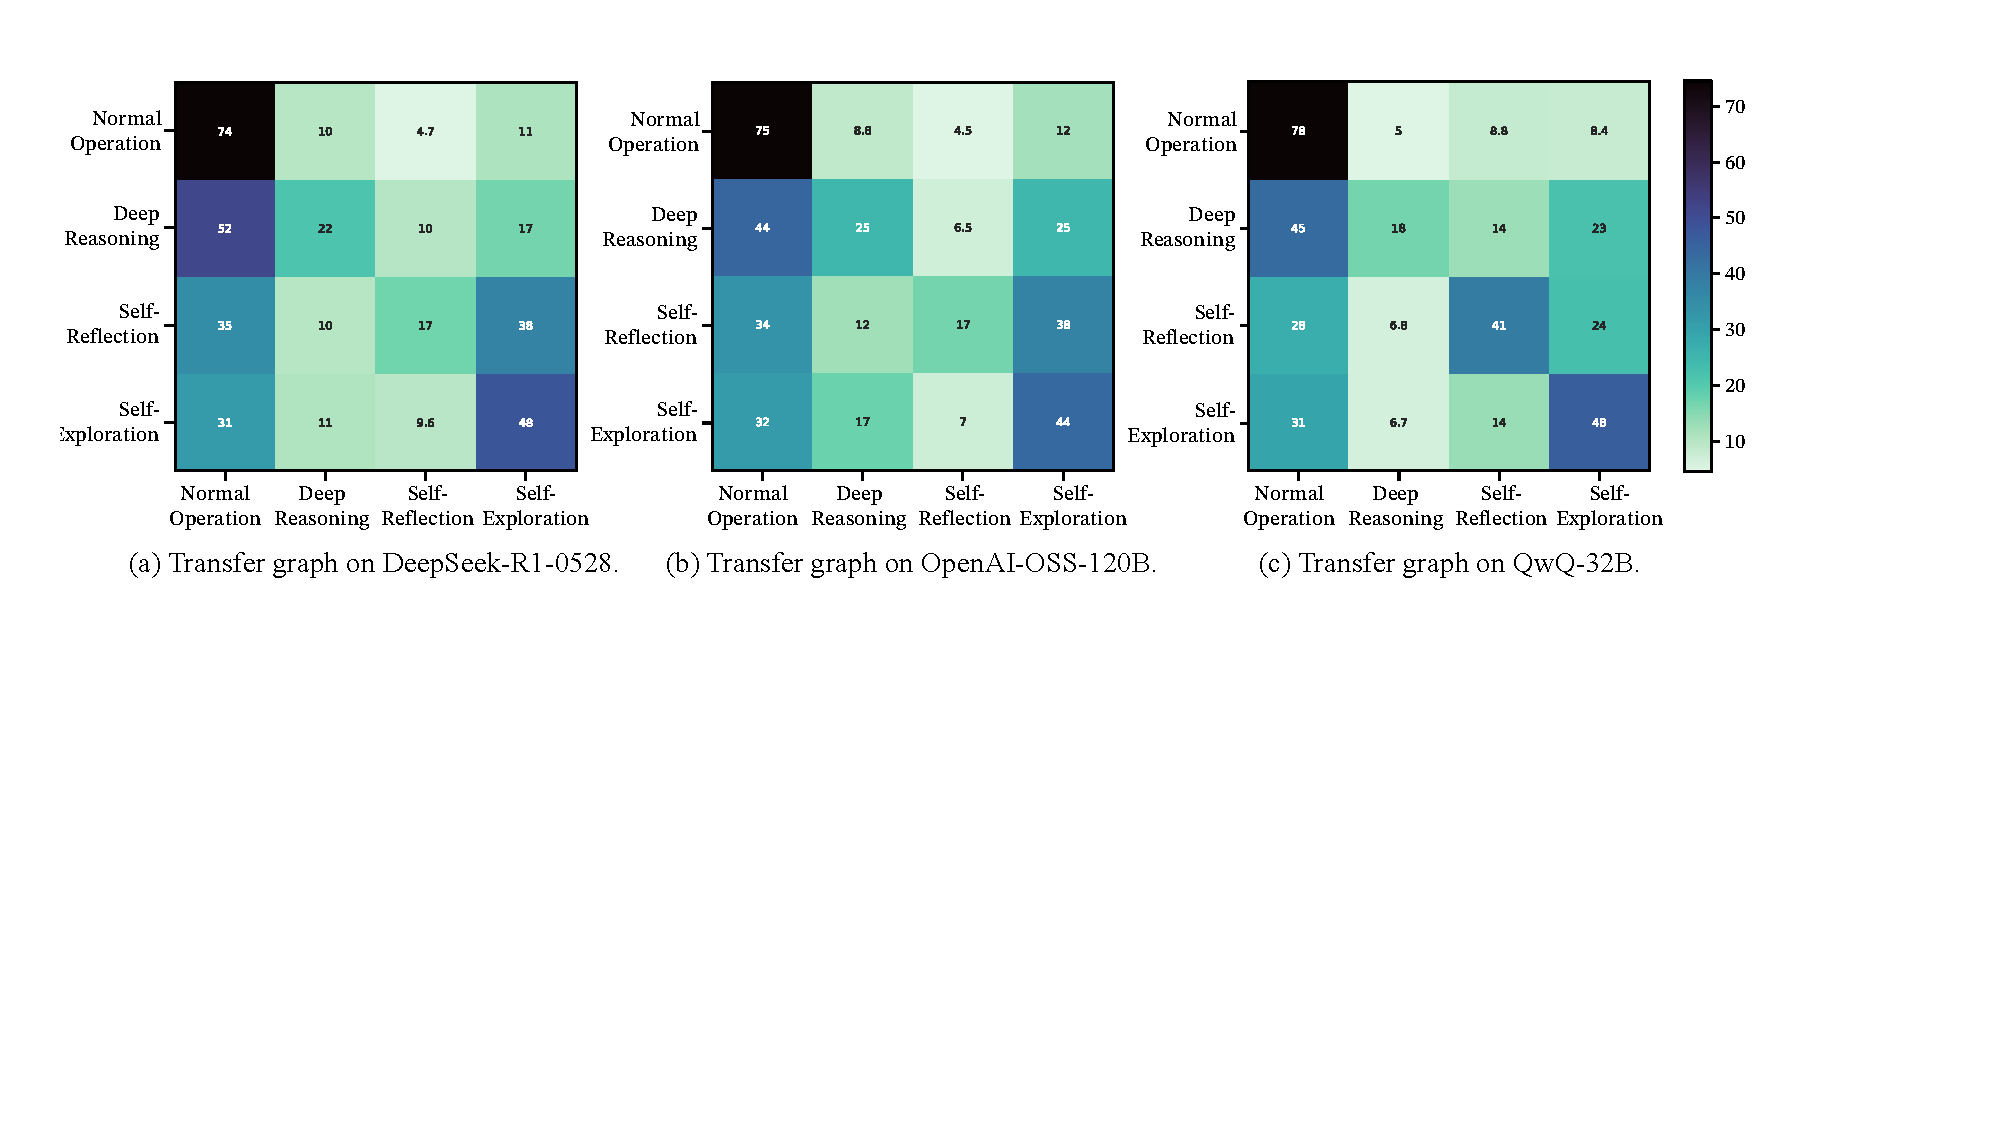
\includegraphics[width=0.98\textwidth]{figures/transfer.pdf}
    \caption{Transfer graph on three different models. Pearson correlation coefficients across models are all greater than 0.9 (p<0.001), when sampling examples > 2,000, transfer graphs will become stable and get over 0.95 Pearson correlation between different sampling sizes.}
    
    \label{fig:transfer}
\end{figure*}

\subsection{Stable Bond Distribution in Long CoT}
To address this, we first verify whether effective Long CoT traces show stable, macromolecular-like organization across models and tasks. As shown in Fig.~\ref{fig:transfer}, traces from multiple LLMs across diverse tasks yield Pearson correlations exceeding 0.9 (p<0.001) for over 2,000 samples. These transfer graphs stabilize with correlations above 0.95 across sampling sizes. This indicates that effective Long CoT structures rely on robust motifs: different models recover similar reasoning topologies across tasks, whereas simple human simulation or ICL cannot emulate the global bond distribution.


\subsection{SFT actually learns these bond structures rather than keywords.}
For the SFT analysis, we consider Llama-3.1-8B-Base that is pre-trained but not instruction-tuned on Long CoT data;
Then, we consider Llama-3.1-8B-Base trained on R1-distilled data as Think-SFT model obtained by supervised fine-tuning enriched with Long CoT traces.\vspace{-8pt}




\begin{figure*}[t]
    \centering
    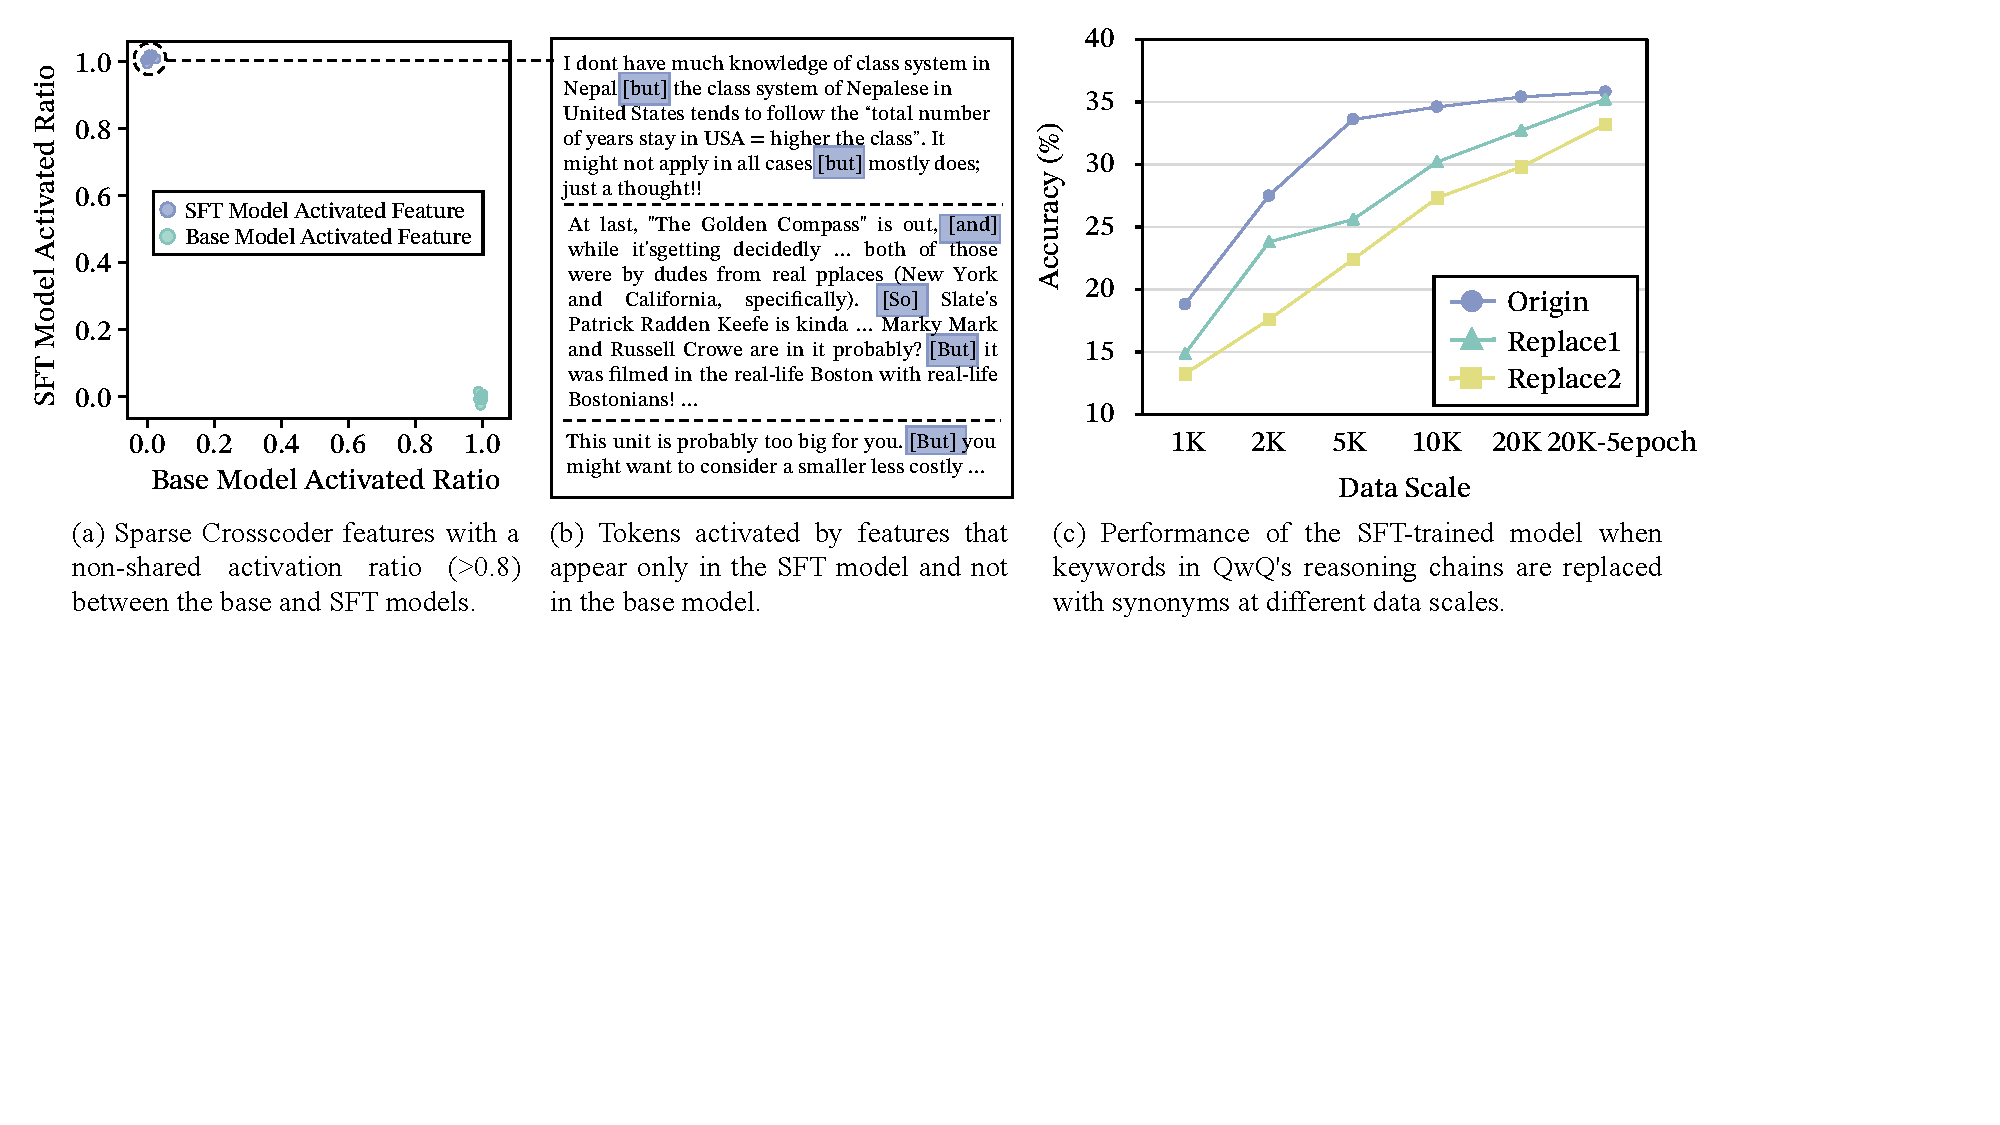
\includegraphics[width=0.98\textwidth]{figures/learning.pdf}
    \caption{The learned features in Long CoT supervised fine-tuning.}
    \label{fig:learning}
\end{figure*}


From a representation-geometry perspective, the sparse auto-encoder analysis shows that Long CoT behavior in the SFT model is concentrated in a small set of discourse-control structures rather than being uniformly distributed across tokens. As shown in Figure~\ref{fig:learning} (a, b), we train a cross-coder sparse auto-encoder that jointly models hidden states from the base model and the Think-SFT model, and then identify features whose activation on think tokens is at least threefold higher than their average activation rate. Within this highly activated subset, many features are predominantly driven by a few connective keywords, such as  \textit{``Maybe''}, \textit{``But / so''}, and \textit{``Alternatively''}, indicating that the SFT process has carved out dedicated latents for managing local hypothesis revision, contrastive moves, and branch selection in long CoT traces.

Based on previous analyses, we argue that models learn the characteristic reasoning behaviors these keywords represent, not the keywords themselves. Following \citet{chen2025towards}, we define three categories of Long CoT reasoning behaviors and test this claim using two training datasets derived from QwQ distillation data. In the first, we replace each keyword with one of four alternative variants. In the second, we remove all keywords while preserving the reasoning trajectories. We then fine-tune identical LLMs on each dataset and evaluate their Long CoT reasoning performance.

As shown in Figure~\ref{fig:learning} (c), explicit keywords like "wait" accelerate learning but are not essential. Models trained without keywords, or with arbitrary alternatives, achieve comparable reasoning performance given sufficient training, provided the underlying reasoning behaviors remain intact. This reveals a fundamental insight: LLMs internalize reasoning structure of reasoning rather than surface lexical cues. Consequently, training data should prioritize the distribution of reasoning behaviors over specific keyword choices to effectively enhance model reasoning capabilities.


However, a key open question remains: do these bonds drive Long CoT structure learning, and if so, \textit{\textbf{why do explicit human imitation or random ICL distillation of these markers often fail?}}







\begin{figure*}[t]
    \centering
    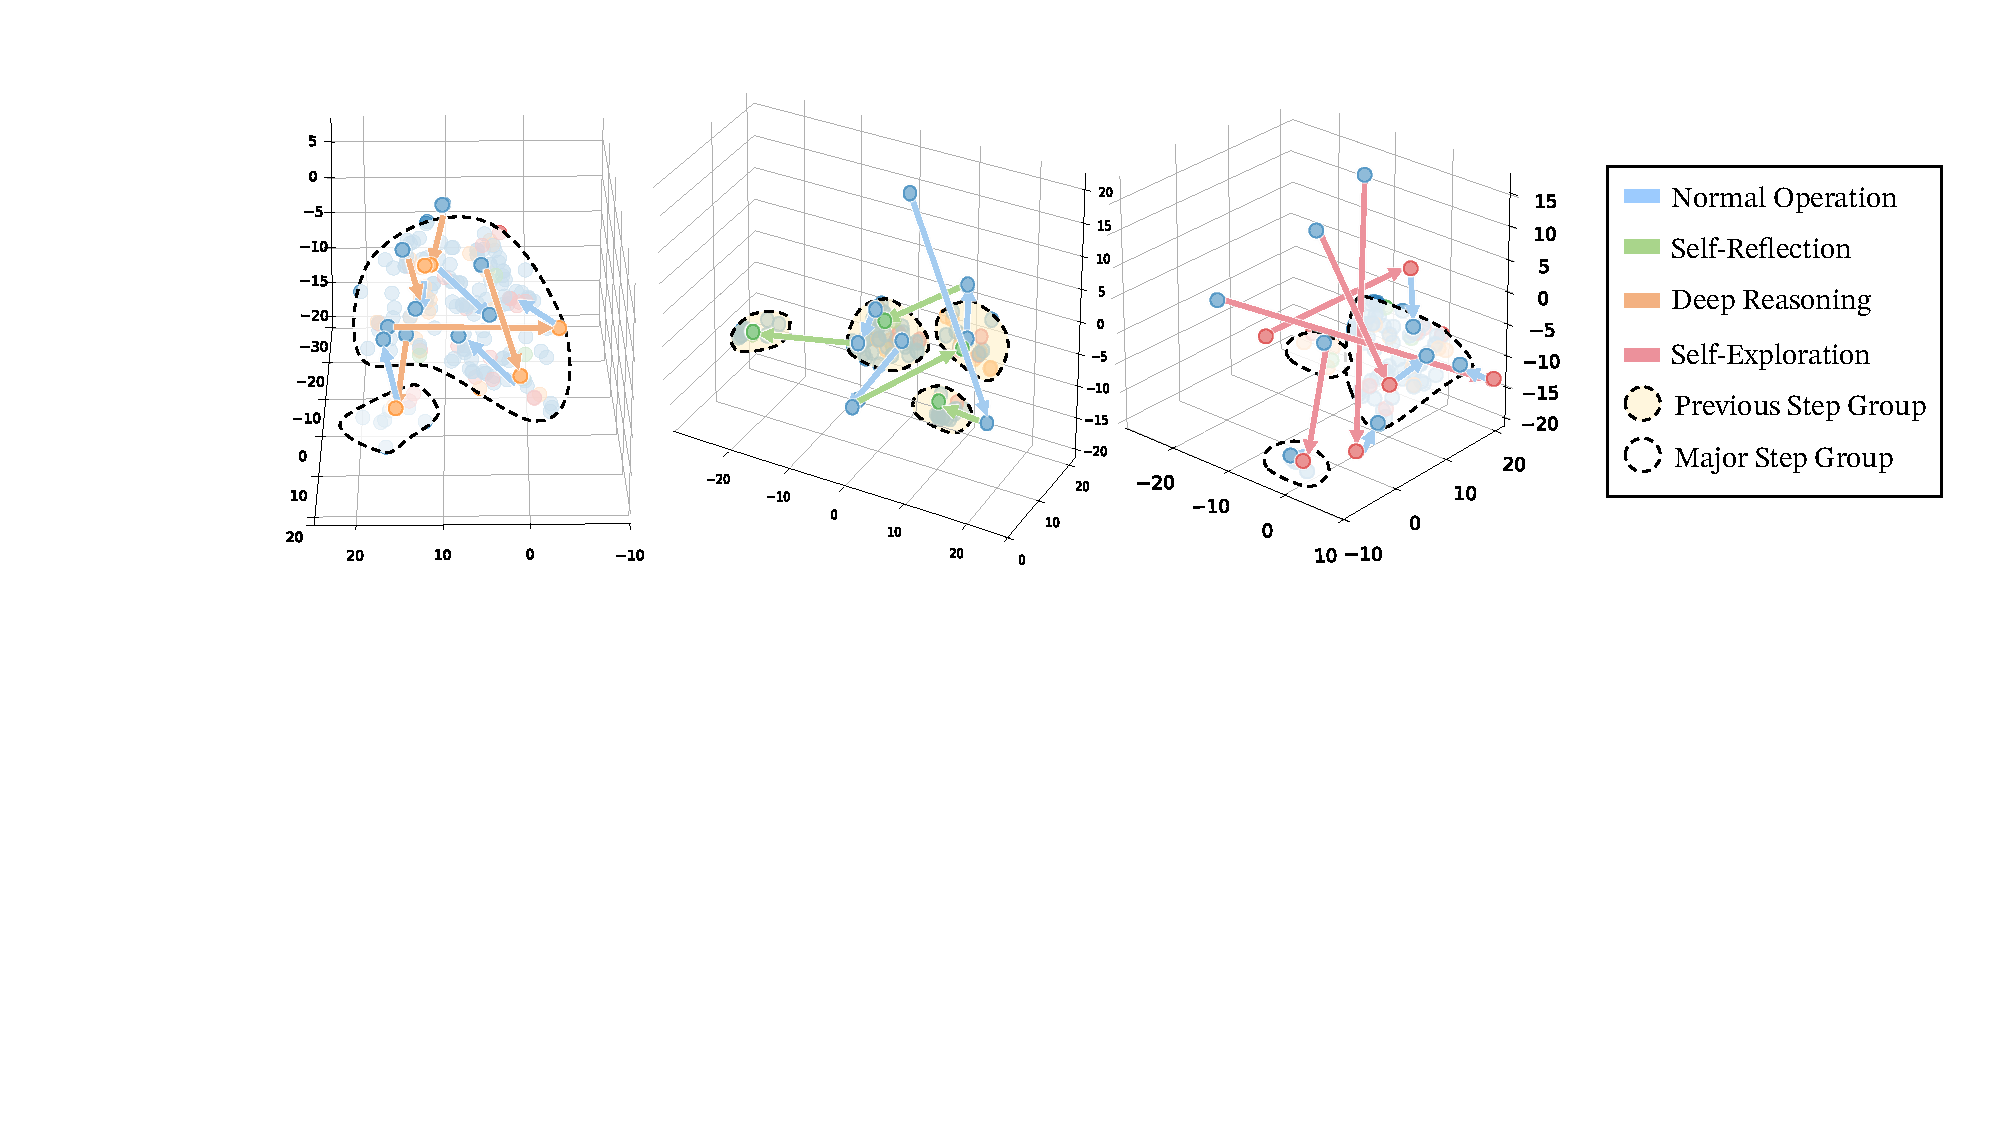
\includegraphics[width=0.96\textwidth]{figures/validation.pdf}
    \caption{Verification of the ``logical folding'' structure on embeddings from Qwen2.5-32B-Instruct and t-SNE-based low-dimensional representations from the OpenAI-OSS-120B-generated reasoning process.}
    
    \label{fig:validation}
\end{figure*}

\begin{figure*}[t]
    \centering
    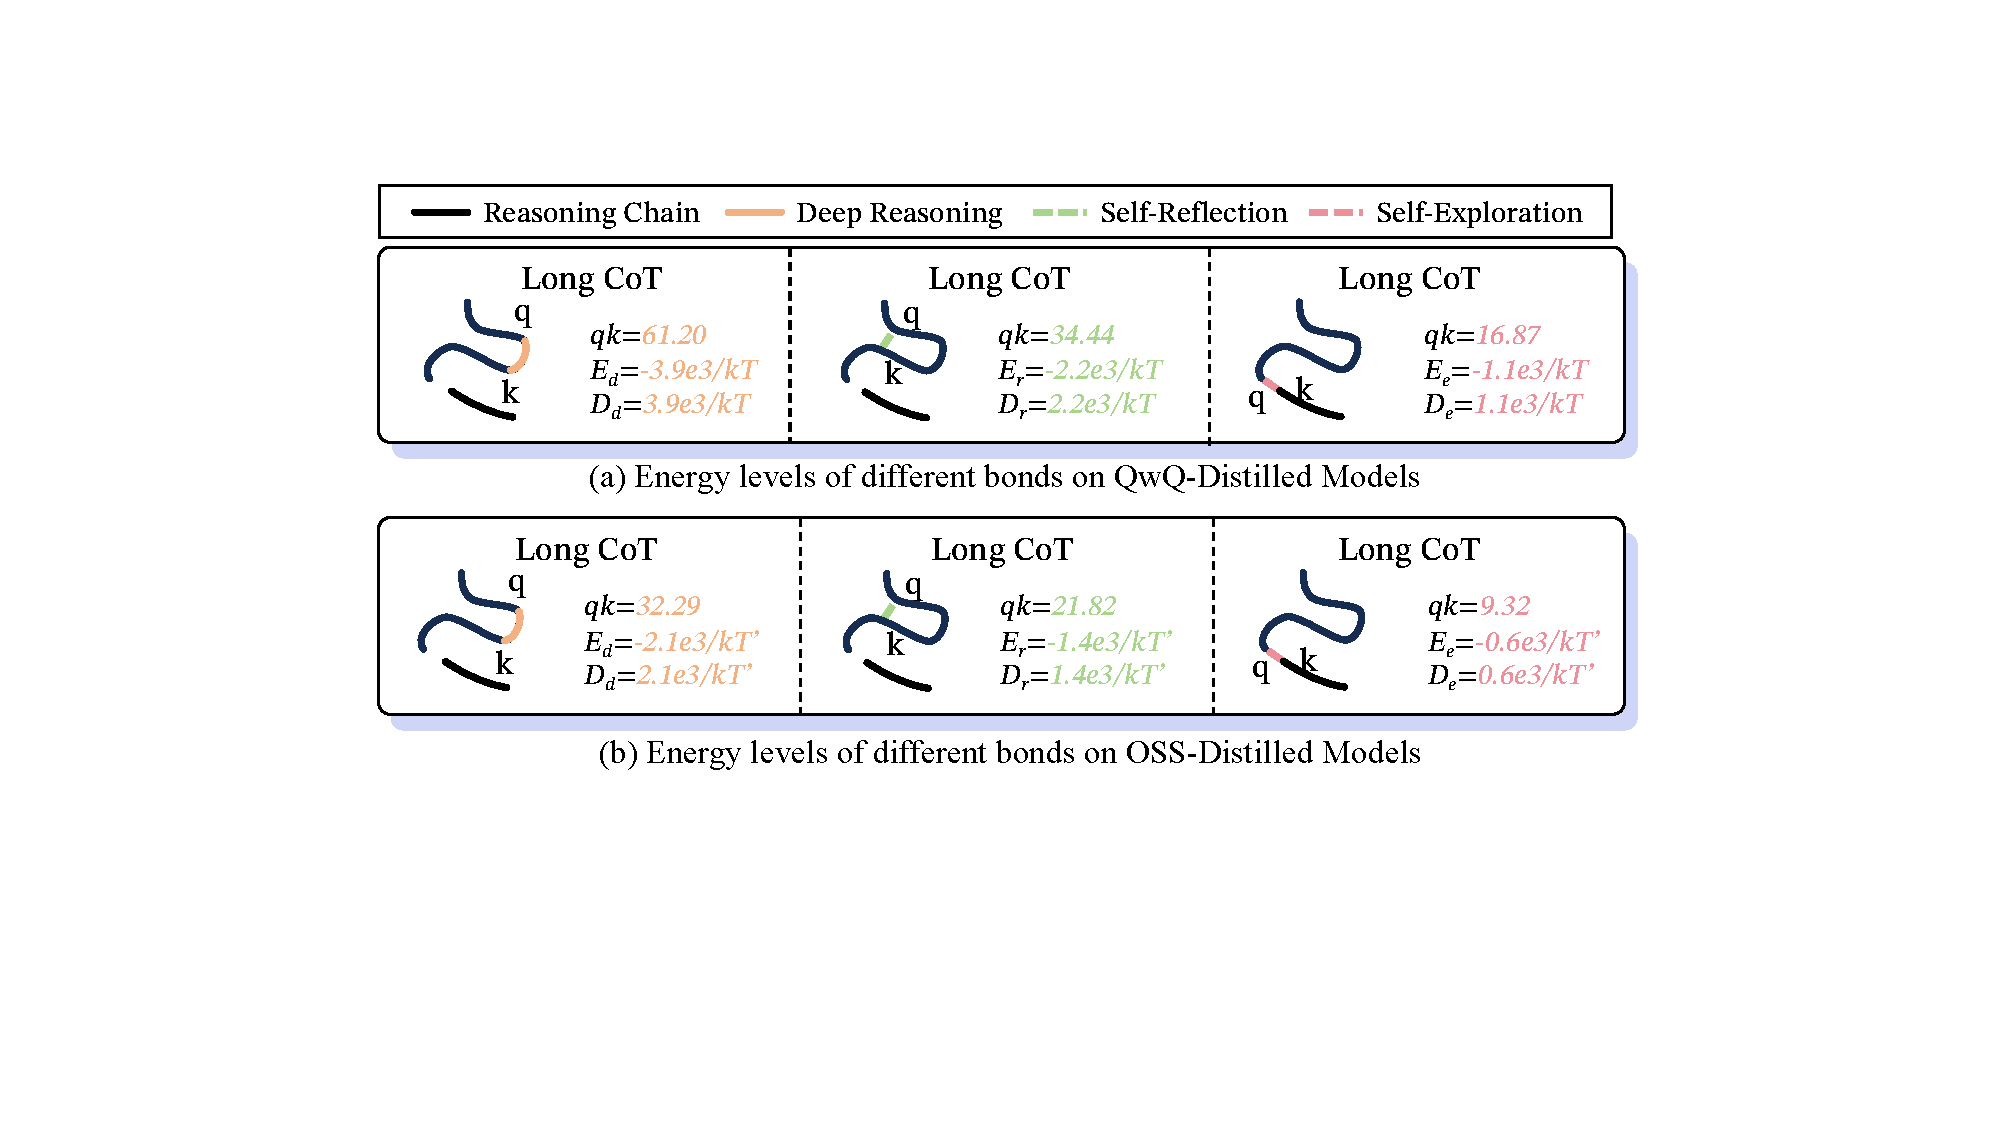
\includegraphics[width=0.76\textwidth]{figures/attention.pdf}
    
    \caption{Energy levels of different bonds across two distilled data.}
    
    \label{fig:attention}
\end{figure*}

\subsection{``Logical Bonding-Folding'' Structure}

To test the hypothesis that Long CoT is analogous to macro-molecular folding, as shown in Fig.~\ref{fig:validation}, we analyzed the topology of CoT in a 3D semantic space. Each trajectory edge was classified as reflection, deep reasoning, or exploration, and its geometric properties were quantified.\vspace{-8pt}






\paragraph{\textbf{Deep-Reasoning stabilizes logical cluster by Covalent Bonding.}}
Modeled as covalent bonds, as shown in Fig.~\ref{fig:validation} (a), deep reasoning bonds mainly increase local connectivity, forming stable subdomains. After deep reasoning, 72.56\% of steps remained within a group distance of less than 3 in the semantic space (generally, group-group distance $>$5.6).\vspace{-8pt}

\paragraph{\textbf{Self-Reflection drives strong folding to previous steps by Hydrogen Bonding.}}
Analogous to hydrogen bonds, as shown in Fig.~\ref{fig:validation} (b), self-reflection transitions fold later steps back onto earlier, semantically similar clusters rather than extending the chain linearly. Quantitatively, 81.72\% of reflection steps reconnected to a previously formed cluster with high semantic similarity.\vspace{-8pt}

\paragraph{\textbf{Self-Exploration gently links different long-distance clusters by Van der Waals Forces.}}
In contrast to local stabilization (Fig.~\ref{fig:validation} (c)), exploration transitions act as loose links between otherwise separated clusters. They show much larger step-to-step distances, with an average trajectory length of 5.32 in the 3D t-SNE projection.
Together, these results suggest that effective Long CoT reasoning is not a simple linear chain; instead, it forms a folded, domain-structured topology consistent with the ``logical folding'' hypothesis.





\subsection{Attention $\Leftrightarrow $ Energy Level of Bonds}
In physical chemistry, the behavior probability with energy level $E_i$ at temperature \(T\) follows the Boltzmann distribution:
\begin{equation}
    P(\text{state}_i) = \frac{\exp\!\big(-E_i / k_B T\big)}{\sum_j {\exp\!\big(-E_j / k_B T\big)}}.
    \label{eq:energy}
\end{equation}
In Transformers, the attention weight \(\alpha_{ij}\) of the \(i\)-th token to the \(j\)-th token is:
\begin{equation}
\alpha_{ij} = \frac{\exp\!\big(q_i \cdot k_j / \sqrt{d_k}\big)}{\sum_l \exp\!\big(q_i \cdot k_l / \sqrt{d_k}\big)}.
\end{equation}
The correspondence follows by defining attention energy \((E)\) \(\leftrightarrow\) \(( - q \cdot k )\), implies lower $E_{ij}$ and thus higher behavior probability.

Formally, our analysis only relies on the observation that attention weights form a Gibbs–Boltzmann distribution over negative logits. We therefore use the term “energy” to denote reparameterized logits and study how their expectations differ across behavior types. 


\begin{table*}[t]
\centering
\resizebox{0.96\textwidth}{!}{%
\begin{tabular}{lcccccccc}
\toprule
    \textbf{Model} & \textbf{GSM8K} & \textbf{MATH-500} & \textbf{AIME2024} & \textbf{AIME2025} & \textbf{AMC2023} & \textbf{OlympiadBench} & \textbf{AVG} \\
    \midrule
    LLaMA-3.1-8B-Base~\citep{dubey2024llama} & 7.58 & 3.20 & 0.00 & 0.00 & 4.22 & 1.19 & 2.70 \\
    \texttt{\ \ + 20K R1-Distill-Data} & 63.38 & 30.60 & 0.21 & 0.42 & 14.22 & 8.30 & 19.52 \\
    \texttt{\ \ + 20K OSS-Distill-Data} & 75.89 & 54.20 & 4.38 & 6.46 & 37.34 & 23.85 & 33.69 \\
    \texttt{\ \ + 20K QwQ-Distill-Data} & 64.53 & 32.20 & 2.92 & 0.42 & 16.72 & 8.89 & 20.95 \\
    \midrule
    Llama-3.1-8B-Instruct~\citep{dubey2024llama} & 75.89 & 35.20 & 4.17 & 1.04 & 23.59 & 12.00 & 25.32 \\
    \texttt{\ \ + 20K R1-Distill-Data}& 79.91 & 60.60 & 2.50 & 3.88 & 33.13 & 23.85 & 33.98 \\
    \texttt{\ \ + 20K OSS-Distill-Data} & 79.00 & 60.80 & 10.83 & 7.71 & 47.03 & 30.22 & 39.27 \\
    \texttt{\ \ + 20K QwQ-Distill-Data} & 82.41 & 60.80 & 4.38 & 8.33 & 32.97 & 25.48 & 35.73 \\
\bottomrule
\end{tabular}
}

\caption{Results across six benchmarks. Full results are reported in Table~\ref{tab:full_distill_result} in the Appendix.}

\label{tab:distill_result}
\end{table*}
We then compare attention energy across Long CoT transition types. Fig.~\ref{fig:attention} shows distinct distributions for deep reasoning, reflection, and exploration. Deep reasoning exhibits the largest effective chemical-bond energy $D_d$. Reflection is intermediate, whereas exploration shows the weakest effective bond energy. This ordering and the relative proportions are consistent across models, supporting the hypothesis that a bond-like mechanism broadly links these reasoning behaviors.





\begin{TakeawayBox}{Takeaway 2}
\begin{itemize}[leftmargin=16pt, itemsep=0pt, topsep=0pt]
    \item Long CoT reasoning exhibits stable structures across models, with reasoning topologies converging.
    \item Semantic isomers, reasoning chains with identical concepts but different logical bonds, succeed or fail based on bond structure, not surface keywords.
    \item Three distinct logical bonds drive CoT structure: reflection folds back to prior clusters, deep reasoning creates stable local domains, and exploration bridges distant concepts, each with characteristic attention energy profiles matching Boltzmann-like distributions.
    \item SFT learns reasoning structure rather than surface keywords, determining Long CoT capability.
\end{itemize}
\end{TakeawayBox}
